%\documentclass[t,handout]{beamer}
\documentclass{beamer}


\usepackage[utf8]{inputenc}
\usepackage[english]{babel}
%\usepackage[tight]{subfigure}
\usepackage{graphicx}
\usepackage{color}
\usepackage{url}
% \usepackage{listings}
%\usepackage[alf]{abntcite}


%\usetheme{Frankfurt} %LEGAL     !!!
% \usetheme{Madrid}     %LEGAL/L%IMPO/COM CAIXA     (sem barra de desenvolvimento)

% \usetheme{Antibes} %NAO
%\usetheme{Berlin} %PODE SER...     (BARRA DE DESENVOLVIMANTO)
% \usetheme{Berkeley}     %FEIO
% \usetheme{Boadilla} %TUDO BRANCO...
% \usetheme{Copenhagen}     %NAO
% \usetheme{Darmstadt} %LEGAL!     !!!
 \usetheme{Dresden}     %LEGAL/LIMPO/SEM CAIXA     (sem caixa fica ruim...)

% \usetheme{Goettingen}     %FEIO DEMAIS!
%\usetheme{Ilmenau} %LEGAL (forte candidato)
% \usetheme{JuanLesPins} %BACANA
% \usetheme{Luebeck}     %FEIO

% \usetheme{Malmoe}     %FEIO
% \usetheme{Warsaw} %NAO...
% \usetheme{Seattle}
% \usetheme{CambridgeUS}
% \usetheme{Singapore}

% \usecolortheme[RGB={130,35,150}]{structure}
% \usecolortheme[RGB={33,33,94}]{structure}
\usecolortheme[RGB={134,153,188}]{structure}
\setbeamertemplate{footline}[frame number]
\setbeamertemplate{navigation symbols}{}

%Hide subsections on teable of contents
%\hypersetup{bookmarksopen=true,bookmarksopenlevel=4}
%\setcounter{tocdepth}{2}



\author[]{\textbf{Leonardo Medeiros}, Hyggo Almeida, Leandro da Silva, Mirko Perkusich and Robert Fischer}

%\date{\today}
\date{20/06/2016}
\institute[]{Federal University Of Campina Grande - BRAZIL
}
\title{A Gait Analysis Approach to Track Parkinson's Disease Evolution Using Principal Component Analysis}
%\logo{\includegraphics[width=0.2\linewidth]{img/logo.png}}
\subtitle{\textbf{CBMS 2016}}

\begin{document}

\begin{frame}
  \titlepage
\end{frame}

% \section{Roteiro}
% \AtBeginSection[]
{\frame{
\frametitle{Summary}
%\tableofcontents
\tableofcontents
}
}






\section{Motivation}
\subsection{}
\begin{frame}{Gait Analysis to Track Parkinson's Disease Evolution}
	\begin{block}{}
	Gait analysis has been strongly applied to evaluate the evolution of neurological diseases such as Parkinson's Disease (PD), which affects about 2$\%$\ of the world population.
	\end{block}

  \begin{block}{}
	In this work, we present a \textbf{reproducible gait analysis to track Parkinson's Disease evolution} by monitoring walking abnormalities. 
  \end{block} 
\end{frame}

\begin{frame}{Gait Analysis}
  \begin{block}{}
  Gait analysis is the systematic study of human locomotion, including qualitative and quantitative assessment.
  \end{block}  
	
	\begin{block}{}
	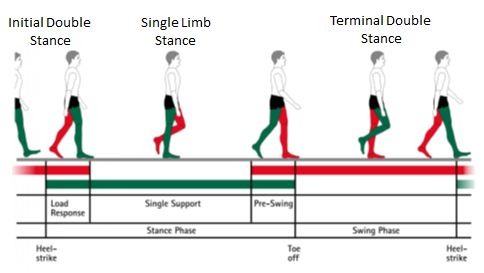
\includegraphics[height=2.2 in]{img/gait-chart.jpg}
	\end{block}
\end{frame}

\begin{frame}{Gait Analysis}
  \begin{block}{}
The human gait is a periodic movement of the limbs during locomotion over a solid substrate. Each gait cycle starts when a foot initiates contact (i.e., heel strike) with the ground and restarts when it touches the ground again.
	\end{block}
\end{frame}

\begin{frame}{Sensors To Acquire VGRF}
  \begin{block}{}
Nowadays, an effective approach is using foot sensors to collect gait data from the forces between the foot and the ground defined as Vertical Ground Reaction Force (VGRF)
  \end{block}
\end{frame}

\begin{frame}{Gait Analysis through VGRF}
  \begin{block}{}
Gait analysis studies the forces and moments of the movement of body segments in a human gait, including the measurement of VGRF. The patients use adapted force sensors under the feet and attached to the shoes to measure the VGRF.
	\end{block}
\end{frame}

\begin{frame}{Motivation}
\begin{block}{}
	Physicians and physiotherapists apply gait analysis \textbf{subjectively in clinical evaluation}, which sometimes is followed by a survey regarding gait quality. This research area has attracted the interest of \textbf{multidisciplinary researchers}.
	\end{block}
\end{frame}

\begin{frame}{PCA for Gait Analysis}
  \begin{block}{}
In this paper, we propose a gait analysis approach to \textbf{track PD evolution by monitoring walking abnormalities}. We \textbf{applied PCA into gait data to detect abnormalities that may indicate the progression of PD}.
  \end{block}
\end{frame}

\begin{frame}{Data Collection}
	\begin{block}{}
	We validated our approach with a public database of foot sensor data, which includes vertical ground reaction force records of healthy subjects and PD patients.
	\end{block}
\end{frame}


\section{PCA for Gait Analysis}
\subsection{}
\begin{frame}{How We Detected Gait Abnormalities ?}
	\begin{block}{}
	We used Principal Component Analysis to identify the gait variance.
	\end{block}
\end{frame}


\begin{frame}{Principal Component Analysis}
	\begin{block}{}
	PCA is a statistic procedure to reduce data and eliminate redundancies. It identifies the data variance and applies linear data transformation to detect the most relevant data components on the first dimension, called the main axis.  The second remaining variance is the secondary axis and so on.
	\end{block}
\end{frame}

\begin{frame}{PCA Step by Step}
	\begin{block}{}
	PCA consists of the following steps: 
		\begin{enumerate}[<+->]
				 \item Scale the measurement data into an \textit{m} x \textit{n} matrix, where \textit{m} is the number of measurement types and \textit{n} is the number of samples;
				 \item Subtract the mean for each measurement type;
				 \item Calculate the \textit{eigenvectors} and \textit{eigenvalues} of the covariance matrix.
				 \item The Calculated \textit{eigenvectors} and \textit{eigenvalues} can be used to project the data into a new space called \textit{eigenspace}.
		\end{enumerate}
	\end{block}
\end{frame}

\begin{frame}{System Overview}
		 \begin{block}{}
			\begin{center}
				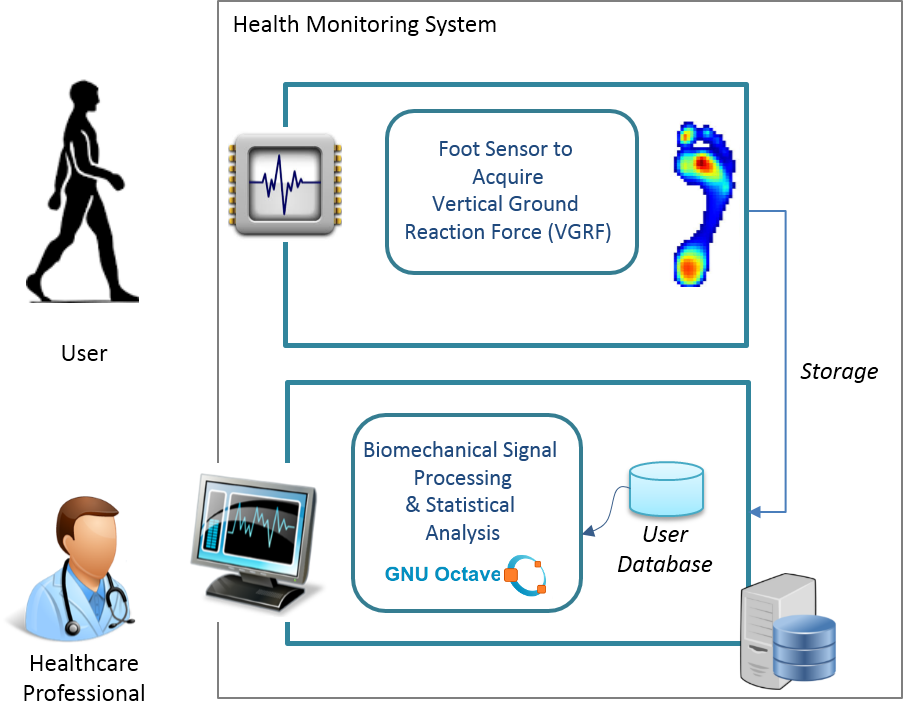
\includegraphics[height=2.2 in]{img/systemoverview.png}
			\end{center}
		 \end{block}
\end{frame}


\begin{frame}{Mean Vector}
		 \begin{block}{}
			\begin{center}
				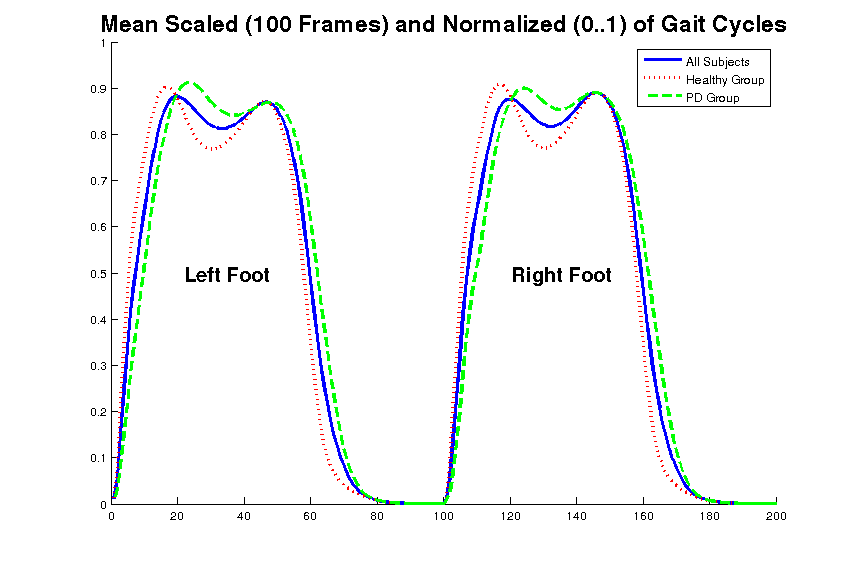
\includegraphics[height=2.2 in]{img/meangait.png}
			\end{center}
		 \end{block}		
\end{frame}

\section{Developed Approach}
\subsection{}
\begin{frame}{Developed Approach}
	\begin{block}{}
	To automate the identification of each gait phase in the VGRF data, it is necessary to use \textbf{signal processing techniques}. 
	\end{block}
	
	\begin{block}{}
	In this work, we focus on the VGRF of each foot and identifying when the foot initiates contact (i.e., start of stance phase) with the ground and when it is off the ground. For this purpose, \textbf{we used the peaks and valleys technique} to identify the beginning and end of each gait cycle.
	\end{block}
\end{frame}

\begin{frame}{Peaks and Valleys}
	\begin{block}{}
		\begin{center}
				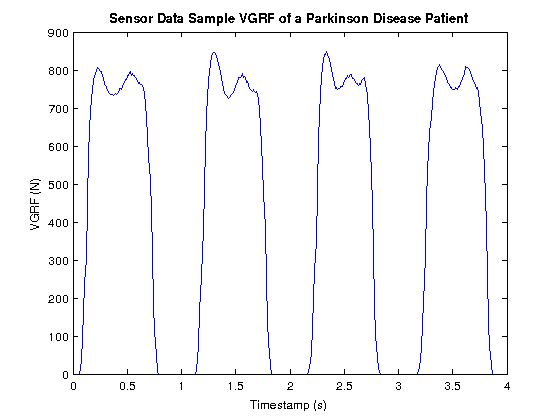
\includegraphics[height=2.2 in]{img/sampleRawData.png}
		\end{center}
	\end{block}
\end{frame}


%\begin{frame}{Biomechanical signal processing}
	%\begin{block}{}
		%\begin{center}
				%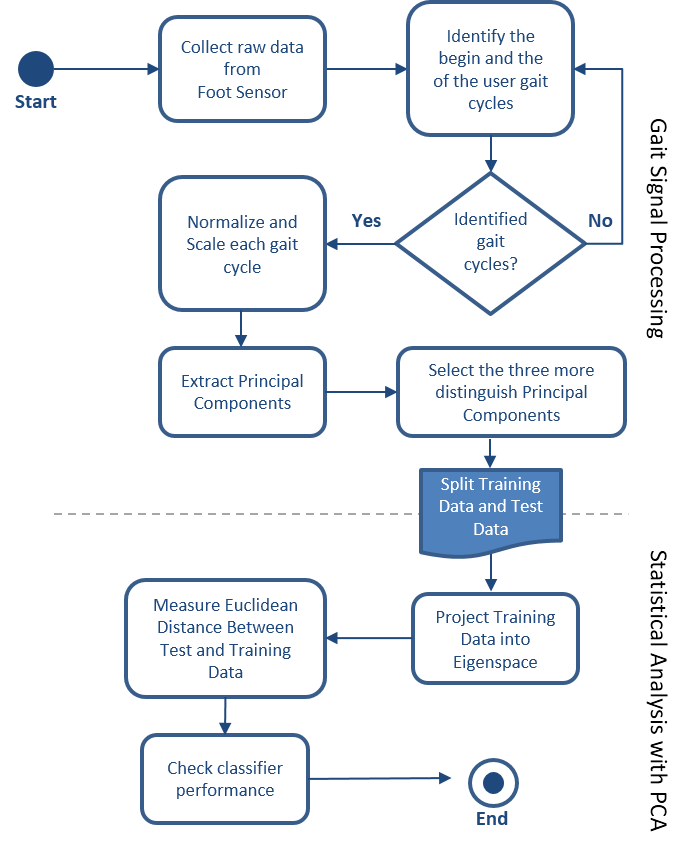
\includegraphics[height=2.2 in]{img/biomecanicalsignal.png}
		%\end{center}
	%\end{block}
%\end{frame}

\begin{frame}{Data Collection}
	\begin{block}
	In this work, we used an database under ODC Public Domain Dedication and License. Available at\textbf{physionet}, which contains the VGRF records of subjects as they walked at their usual pace for approximately 2 minutes on level ground. 
	\end{block}
\end{frame}

\section{Validation}
\subsection{}
\begin{frame}{PCA for Gait Analysis Data Classification}
	\begin{block}{}
		\begin{itemize}[<+->]
			\item PCA defines an orthogonal linear transformation that transforms data into a new coordinate system in which the greatest variance by any projection of data;
			\item We project this data creating a new space;
			\item So, we used the euclidean distance of the test data to the training data to classify each subject as \textbf{PD's Group or Control Group}.
		\end{itemize}
	\end{block}
\end{frame}


\begin{frame}{Projection of PD's (RED) and HEALTHY (BLUE dots)}
	\begin{block}{}
		\begin{center}
				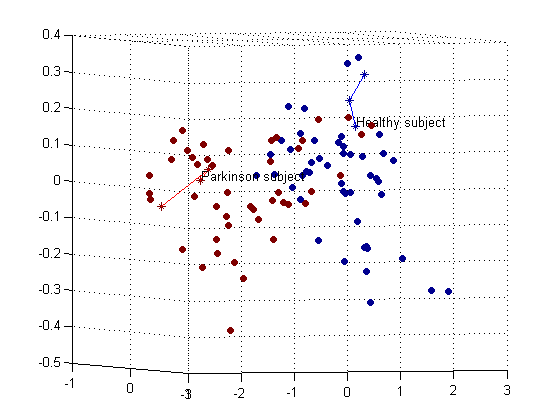
\includegraphics[height=2.6 in]{img/pca-projection-health-parkinson.png}
		\end{center}
	\end{block}
\end{frame}

\begin{frame}{PCA with Euclidean Distance Classifier Performance}
   \begin{block}{}
   
   \begin{columns}[c]
     \begin{column}{0.5\linewidth}
				\begin{table}[!htbp]
					\centering
					\begin{tabular}{l|c|c|}
					\cline{2-3}
					\multicolumn{1}{c}{}                         & \multicolumn{2}{|c|}{\textit{\textbf{Predictive Class}}} \\ \cline{2-3} 
																											 & \textbf{Parkinson}      & \textbf{Control}         \\ \hline
					\multicolumn{1}{|l|}{\textbf{Parkinson}} & 43       & 7           \\ \hline
					\multicolumn{1}{|l|}{\textbf{Control}}     & 12           & 38     \\ \hline
					\end{tabular}
			\end{table}

     \end{column}

     \begin{column}{0.55\linewidth}
						\begin{table}[htbp!]
						\begin{tabular}{|l|r|}
						\hline
						\multicolumn{2}{|l|}{\textbf{Classifier Metrics}} \\ \hline
							\textbf{TpRate}                    & 86.00$\%$\                 \\ \hline
							\textbf{FpRate}                    & 24.00$\%$\                \\ \hline
							\textbf{Precision}                 & 78.18$\%$\                \\ \hline
							\textbf{Accuracy}                  & 81.00$\%$\                \\ \hline
							\textbf{F-Score}                 & 81.90$\%$\                \\ \hline
						\end{tabular}
						\end{table}
    \end{column}
\end{columns}
\end{block}
\end{frame}



%===========================================================================================
%
%\begin{frame}{Parkinson Disease (PD)}  
  %\begin{block}{}
%The symptoms associated with PD are caused by a \textbf{degeneration of dopaminergic neurons} in the substantia nigra. Common treatment focuses on \textbf{drugs that activate dopamine receptors}. However, the medication's effectiveness decreases over the years \textbf{requiring higher dosages}
  %\end{block} 
%\end{frame}
%
%\begin{frame}{PD's Treatment and Disease Management} 
    %\begin{block}{}
      %\begin{itemize}
					%\item Clinical trial evaluation: subjectively and sporadically;
					%\item Motor fluctuations (\textit{on/off} phenomenon).
     %\end{itemize}
  %\end{block}
%\end{frame}
%
%
%
  %
%
%
%\section{Objectives}
%\subsection{}
%\begin{frame}{Main Objective}
		 %\begin{block}{}
				%A non-invasive HMS for Parkinson's Disease motor symptoms based on games to continuously provide data regarding patient, without reminding the disease's treatment
		 %\end{block}
     %\begin{block}{}
     %\begin{center}		
		%
      %\end{center}
    %\end{block}
		%\begin{alertblock}{}
		%The monitoring at the patients' home provides more data regarding the patient's symptoms and improves the medication management mainly in the disease's intermediate stages
 	%\end{alertblock}
%\end{frame}
%
%\begin{frame}{Main Requirements}
    %\begin{block}{}
		    %\begin{enumerate}[<+->]
            %\item A contactless measurement of patient motor symptoms inside the game environment;
						%\item Use of a popular consumer electronic device as input to have a non-invasive, cost-effective solution for home use.
        %\end{enumerate}
    %\end{block}
%\end{frame}
%
%
%\begin{frame}{Who will use the Game-Based Health Monitor Approach}
    %\begin{block}{}
        %\begin{itemize}[<+->]
            %\item A person with age above 55 years old;
            %\item A person with Parkinson's disease;
            %\item Neurologist and physiotherapist responsible for patient's treatment.
        %\end{itemize}
    %\end{block}
%\end{frame}
%
%
%\begin{frame}{Use Scenario}
   %\begin{block}{}
      %\begin{itemize}[<+->]
       %\item A PD' patient play the HGM Client in home and seamlessly provide the motor data;
       %\item So, the motor signs are sent to HGM Server;
       %\item The HGM Server process the user's data and identify the occurrence of the PD's disease bradykinesia symptom;
       %\item Then, the neurologist visualize the user's health information to assess the patient's level of motor deficiency.
      %\end{itemize}
  %\end{block}
%\end{frame}
%
%\begin{frame}{System Overview}
		 %\begin{block}{}
			%\begin{center}
				%\includegraphics[height=2.2 in]{img/systemoverview3.png}
			%\end{center}
		 %\end{block}
%\end{frame}
%
%
%\begin{frame}{What was developed?}
    %\begin{block}{}
        %\begin{itemize}[<+->]
            %\item  A semi-structured interview with healthcare professionals associated to scientific references to identify the system requirements;
            %\item The development of the Health Game Monitor (HGM) Client (Catch the Spheres' game);
            %\item The development of the HGM Server, responsible for processing the data and making the results available to the health professional;
						%\item Experimental studies with target users.
        %\end{itemize}
    %\end{block}
%\end{frame}
%
%\section{System Requirements}
%\subsection{}
%\begin{frame}{Qualitative Research Analysis} 
    %\begin{block}{}					
		%The respondents suggested focusing on the bradykinesia motor symptom due to its debilitating progress. Thus, treatment benefits could be correlated with the \textbf{increase of amplitude and angular velocities of an arm's adduction and abduction movements}.
    %\end{block}
%\end{frame} 
%
%
%
%
%\begin{frame}{Some Elicited Requirements}
	%\begin{block}{}
		%\begin{itemize}[<+->]
			%\item	Easy and safe to use equipment
      %\item Incite the player to perform specific movements that are required for the measurement 
      %\item Game with clear and entertaining goal and adapted to the user's skills
			%\item Provide a informative visual way to the healthcare professional
		%\end{itemize}
	%\end{block}
%\end{frame}
%
%
%
%
%\section{System Development}
%\subsection{}
%\begin{frame}{System Architecture}
		 %\begin{block}{}
			%\begin{center}
				%\includegraphics[height=2.2 in]{img/systemarchitecture3.png}
			%\end{center}
		 %\end{block}
%\end{frame}
%
%
%\begin{frame}{The Biomechanical Analysis of Human Movement}
  %\begin{block}{}
   %The diagnosis and treatment process for PD uses the biomechanical analysis of human movement, where the patients are asked to lift their arms, one after the other, at the highest amplitude and velocity they are able to, in order to check the bradykinesia progress. 
  %\end{block}
%\end{frame}
%
%\begin{frame}{Ms-Kinect Joints Acquisition}
  %\begin{block}{}
      %\center \includegraphics[height=2.5 in]{img/articulacoes-sel.png}
			%\caption{Modificações no Jogo ao Longo das Fases de Desenvolvimento~\cite{fullerton2008game}}
  %\end{block}
	%
	%\begin{block}{}
	%Adduction and Abduction involves: \textbf{wrist, shoulder, and hip} joints.
	%\end{block}	
%\end{frame}
%
%
%
%\begin{frame}{Angle over time with the peak and valley detection technique}
  %\begin{block}{}
      %\center 
      %\includegraphics[height=1.6 in]{img/signalamplitudepeakvaley-2.png}
  %\end{block}
	%
	%\begin{block}{Angular motion calculation}
	%The cycle movement and transform the MS-Kinect data into angles. Thus, we calculate the \textbf{angular motion} of the adduction and abduction movements.
	%\end{block}
%\end{frame}
%
%\begin{frame}{Some Elicited Requirements}
	%\begin{block}{}
		%\begin{itemize}[<+->]
			%\item	Easy and safe to use equipment
      %\item Incite the player to perform specific movements that are required for the measurement 
      %\item Game with clear and entertaining goal and adapted to the user's skills
			%\item Provide a informative visual way to the healthcare professional
		%\end{itemize}
	%\end{block}
%\end{frame}
%
%\begin{frame}{Developed Health Game Monitor: Catch the Spheres}
	%\begin{center}
      %\center \includegraphics[height=2.2 in]{img/catch_colour.png}
	%\end{center}
%\end{frame}
%
%\section{Experiments}
%\subsection{}
%\begin{frame}{Case Control Study}
	%\begin{block}{}
	%A total number of 30 subjects participated where 15 subjects for each group.
		%\begin{itemize}
			%\item PD' Group: 10 men and 5 women, between 51 and 65 years (mean: 58);
			%\item Control Group: 11 men and 4 women, between 50 and 65 years (mean: 57).
		%\end{itemize}
	%\end{block}
%\end{frame}
%
%\begin{frame}{Procedure for Data Collection}
	%\begin{block}{}
	%\begin{compactenum}
	%\item The subject stands at distance of 2 meters from the motion sensor at a place marked for that purpose on the ground;
	%\item The subject faces a projection of the game on a wall, centered over the motion sensor;
	%\item The subject plays the game \textit{Catch the Spheres} for 5 minutes;
	%\item The subjects end the game by reaching the virtual exit button.
%\end{compactenum} 
	%\end{block}
%\end{frame}
%
%
%\begin{frame}{Data Classifier: SVM}
%\begin{block}{}
	%In this work, we used Support Vector Machine (SVM) as the supervised learning method. SVM seeks to find a margin that separates all positive and negative example.
		%
	%We choice this algorithm because he has \textbf{a good generalization to discriminate between two classes}.
%\end{block}
%\end{frame}
%
%
%\begin{frame}{SVM Parameter Optimization}
%\begin{block}{}
%In this work, we applied the grid search technique to identify the best SVM parameters, using Leave-One-Out Cross-Validation (LOOCV).
%\end{block}
%\end{frame}
%
%

%
%
%\subsection{User Acceptance}
%\begin{frame}{Goal Question Metric (GQM) for User Acceptance}
	%\begin{block}{}
	%Based on the GQM paradigm, we defined two goals:
		%\begin{description}
			%\item [G1]: Analyze our HMS PD approach for the purpose of evaluating with respect to usability from the view point of the patients in the context of the game \emph{Catch the Spheres}
			%\item [G2]: Analyze our HMS PD approach for the purpose of evaluating with respect to fit to daily routine from the view point of the patients in the context of the game \emph{Catch the Spheres}
		%\end{description}
	%\end{block}
%\end{frame}
%
%
%\begin{frame}{GQM Results}
	%\begin{block}{}
	%The measurements were collected we obtained the following result indicating:
		%\begin{itemize}
			%\item 90\% of the users felt motivated with the game;
			%\item 80\% would add this game-based monitoring approach into their daily routine; 
			%\item 75\% considered it safe for elderly users.
		%\end{itemize}
	%\end{block}
%\end{frame}
%
%\section{Conclusion}
%\subsection{}
%\begin{frame}{Conclusion}
	%\begin{block}{}
	%In this work we presented a game-based approach to monitor with a symptom classification \textit{Precision} of 92.31\%. Moreover, 90,00\% of the patients considered our approach non-invasive and easy to integrate into their routine. 
	%\end{block}
%\end{frame}
\section{Questions}
\begin{frame}{Questions}
	\begin{block}{Reproducible Research}
	Our source code is under GPL License Version 3.0 and can be reproduced using an Open Source Application for numerical computations (Octave Version 3.8.1). 
	\end{block}

	\begin{block}{Source Code and Relevant Data}
	To reproduce our results we created a web page containing all the relevant information~\url{http://gaitparkinson.wordpress.com}. 
	\end{block}
\end{frame}

\bibliographystyle{IEEEtran}
\bibliography{sigproc2,IEEEFormat}

\end{document}
	